\task{7.1}{Predicting the observed convergence order}
Task 5.5 gives first-order time error and second-order space error. For a stable method on a
smooth problem over a fixed time interval, the corresponding global estimate has the form
\[
E\le C_t\Delta t+C_xh^2+C_yh^2,
\]
with constants independent of the refined mesh sizes. Keeping
$r=\alpha\Delta t/h^2$ fixed means
\[
\Delta t=\frac{r}{\alpha}h^2.
\]
Substitute this relation into the error estimate:
\[
E\le\left(C_t\frac r\alpha+C_x+C_y\right)h^2.
\]
Therefore
\[
\boxed{E(h)=O(h^2),\qquad p_{\mathrm{predicted}}=2.}
\]
On halving $h$, the time step is quartered. Both time and spatial errors then decrease by
approximately four. Equivalently,
\[
\log_2\frac{E(h)}{E(h/2)}\longrightarrow2.
\]
This does not make forward Euler second order in time: its time error is still $O(\Delta t)$,
but the chosen refinement path makes $\Delta t$ proportional to $h^2$.
A special solution and parameter can cancel the leading error and produce an unusually high
observed order; the generic expectation remains two. Choosing $r=0.2$ in the next task avoids
the leading-error cancellation for the verification mode.

\task{7.2}{Convergence study}
\partsol{a}
We use the prescribed verification problem on $[0,1]^2$:
\[
u_0(x,y)=\sin(\pi x)\sin(\pi y),\qquad u=0\text{ on all four edges},\qquad\alpha=1,
\]
with exact solution
\[
u_{\mathrm{exact}}(x,y,t)=\sin(\pi x)\sin(\pi y)e^{-2\pi^2t}.
\]
The final time is $T=0.05$ and the fixed time-step parameter is $r=0.2<1/4$.
For each $N\in\{16,32,64,128,256\}$, set
\[
h=\frac1N,\qquad \Delta t=\frac{0.2}{N^2},\qquad
M=\frac{T}{\Delta t}=\frac{N^2}{4}.
\]
Every requested $N$ is even, so $M$ is an integer. Thus we keep $r$ exactly fixed and reach
the same $T$ exactly in the mathematical parameter specification, without rounding the step count.

\textbf{Implementation procedure.}
\begin{enumerate}
\item Allocate two contiguous double-precision arrays of $(N+1)^2$ values.
\item Initialize interior nodes from the sine product. Set all boundary entries to exactly zero
in both arrays; do not rely on floating-point evaluation of $\sin\pi$.
\item Apply the seven-operation update in Task 5.2(d) to every interior node for $M$ steps.
\item Swap the two array buffers after each step, keeping the old level intact during the update.
\item Evaluate the exact solution at the same nodes and final time, then compute both error norms.
\end{enumerate}
The reference program is C++17, compiled with optimization and floating-point contraction disabled.
It computes the full grid at every step; the table below is not generated solely from a modal formula.

\partsol{b}
Define the nodal error and the requested norms by
\[
e_{i,j}=u^M_{i,j}-u_{\mathrm{exact}}(x_i,y_j,T),
\]
\[
\norminf e=\max_{0\le i,j\le N}|e_{i,j}|,
\qquad
\normh e=\left(h^2\sum_{i=0}^N\sum_{j=0}^N e_{i,j}^2\right)^{1/2}.
\]
The factor $h^2$ makes the squared norm a quadrature approximation of a continuous integral.
Without it, changing the number of nodes would change the scale of the norm artificially.
Here the boundary errors are zero.

The observed order in a row compares that row with the preceding coarser grid, using
$\normh e$:
\[
p_{\mathrm{obs}}(N)=\log_2\frac{E(N/2)}{E(N)}.
\]
\begin{center}
\small
\begin{tabular}{rrrrrr}
\toprule
$N$ & $h$ & Steps & $\norminf e$ & $\normh e$ & $p_{\mathrm{obs}}$\\
\midrule
\tableinput{tables/task_7_2.tex}
\bottomrule
\end{tabular}
\end{center}
The time steps are, respectively,
\[
7.8125\times10^{-4},\quad1.953125\times10^{-4},\quad4.8828125\times10^{-5},
\]
\[
1.220703125\times10^{-5},\quad3.0517578125\times10^{-6}.
\]
\begin{figure}[H]
\centering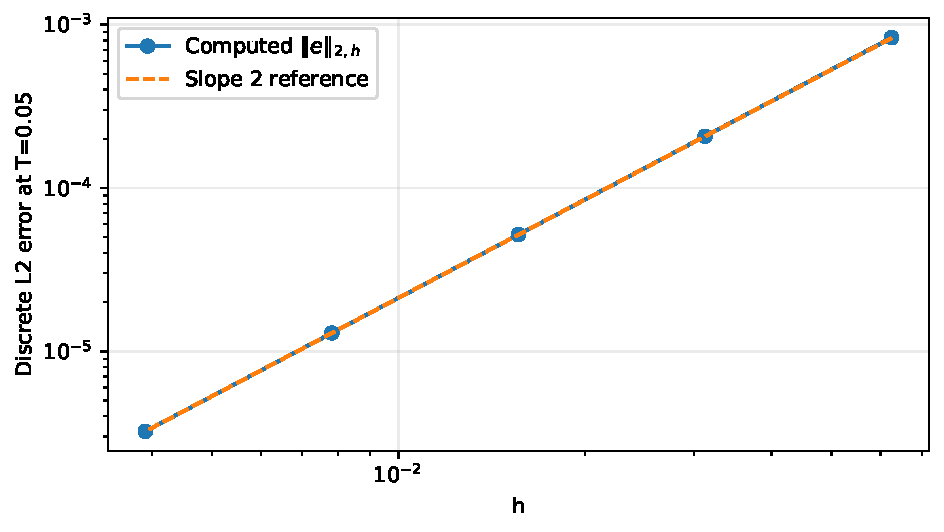
\includegraphics[width=.88\linewidth]{task_7_2_convergence.pdf}
\caption{Computed discrete $L^2$ error versus grid spacing at $T=0.05$, $r=0.2$.
The dashed line is proportional to $h^2$. Both axes are logarithmic.}
\end{figure}

\textbf{Independent analytical check of the computed table.}
For this initial condition, the sampled sine product is an eigenvector of the discrete Laplacian.
Its per-step factor is
\[
G_N=1-8r\sin^2\!\left(\frac{\pi}{2N}\right).
\]
Therefore, in exact arithmetic,
\[
u_{i,j}^M=G_N^M\sin\!\left(\frac{\pi i}{N}\right)
\sin\!\left(\frac{\pi j}{N}\right).
\]
Write $A_N=G_N^M-e^{-2\pi^2T}$. Then
$e_{i,j}=A_N\sin(\pi i/N)\sin(\pi j/N)$.
Because every $N$ in the table is even, the centre node has both sine factors equal to one:
\[
\norminf e=|A_N|.
\]
Also,
\[
\sum_{i=1}^{N-1}\sin^2\!\left(\frac{\pi i}{N}\right)=\frac N2.
\]
One way to see this is to use $\sin^2z=(1-\cos2z)/2$ and the vanishing sum of the $N$th
roots of unity. Applying this identity in both directions gives
\[
\normh e^2=h^2A_N^2\left(\frac N2\right)^2=\frac{A_N^2}{4},
\qquad
\boxed{\normh e=\frac12\norminf e.}
\]
The full-grid numerical results satisfy these modal predictions to within $5\times10^{-13}$
in absolute difference. This checks the stencil, step count, exact-solution evaluation, and
the normalization of the error norms independently of the observed slope.

\partsol{c}
The orders $2.00577$, $2.00144$, $2.00036$, and $2.00009$ approach two, as predicted in
Task 7.1. Both norms decrease by approximately a factor of four under each refinement.
The data therefore verify the expected convergence behaviour for this test.

The leading error can also be derived explicitly. For $h=1/N$,
\[
G_N=1-2r\pi^2h^2+\frac{r\pi^4}{6}h^4+O(h^6),
\]
so
\begin{align*}
\log G_N
&=-2r\pi^2h^2+\left(\frac r6-2r^2\right)\pi^4h^4+O(h^6),\\
M\log G_N
&=-2\pi^2T+\pi^4T\left(\frac16-2r\right)h^2+O(h^4),
\end{align*}
where $M=T/(rh^2)$. Consequently,
\[
A_N=e^{-2\pi^2T}\pi^4T\left(\frac16-2r\right)h^2+O(h^4).
\]
For $r=0.2$ this coefficient is nonzero and negative, so the leading error is truly second
order and the numerical mode decays a little faster than the exact one. For the special value
$r=1/12$, the leading error of this particular mode cancels; that is why a generic parameter
is preferable when using one exact mode to check the scheme's ordinary order.

\task{8.1}{Why an in-place update changes the method}
Assume rows are visited in increasing $j$, and columns within each row in increasing $i$.
Only the interior is updated; prescribed Dirichlet boundary values remain fixed.

\partsol{a}
When node $(i,j)$ is reached:
\begin{itemize}
\item The west neighbour $(i-1,j)$ has already been visited in the current row, so an interior
west neighbour contains level $n+1$ data.
\item The south neighbour $(i,j-1)$ belongs to an earlier row and also contains level $n+1$ data
when it is an interior unknown.
\item The east neighbour $(i+1,j)$ and north neighbour $(i,j+1)$ have not yet been visited,
so they still contain level $n$ data.
\item The centre still contains its old value until this update overwrites it.
\end{itemize}
At the first interior row or column, the corresponding south or west neighbour may instead
be a fixed boundary value. The issue concerns neighbours that are themselves updated unknowns.

\partsol{b}
Using one array would therefore apply the mixed-level relation
\[
u_{i,j}^{\mathrm{new}}=u_{i,j}^{\mathrm{old}}+r\left(
u_{i-1,j}^{\mathrm{new}}+u_{i+1,j}^{\mathrm{old}}
+u_{i,j-1}^{\mathrm{new}}+u_{i,j+1}^{\mathrm{old}}
-4u_{i,j}^{\mathrm{old}}\right).
\]
This is \emph{not} the forward-Euler scheme derived in Task 5.2, whose right-hand side must
use only level $n$. Reversing the traversal changes which neighbours are new, so the result
depends on the visitation order.

For a concrete example, consider the 1D three-interior-node row with zero endpoint values,
initial interior values $(1,0,0)$, and $r=0.1$:
\begin{center}
\begin{tabular}{lr}
\toprule
Update method & New interior values\\
\midrule
Correct simultaneous explicit update & $(0.8,\ 0.1,\ 0)$\\
In place, left to right & $(0.8,\ 0.08,\ 0.008)$\\
In place, right to left & $(0.81,\ 0.1,\ 0)$\\
\bottomrule
\end{tabular}
\end{center}
For example, in the left-to-right pass the second node reads the already changed first node,
so it receives $0.1\times0.8=0.08$ instead of $0.1\times1=0.1$.
The three different results demonstrate both the change in method and the order dependence.

\partsol{c}
When the domain is divided among processes, each process updates its own nodes, and their
relative execution order is not fixed. A valid explicit step must produce the same mathematical
result regardless of which process runs first. If updates read a mixture of old and new values,
the output depends on process boundaries, scheduling, and communication timing.

Use two arrays: read all stencil values from \texttt{old}, write all updated nodes into
\texttt{next}, then swap their buffers after the step. The swap exchanges array storage references;
it does not copy the full field. With consistent arithmetic order and correctly refreshed halos,
this preserves the serial update independently of how the grid is partitioned.

\task{8.2}{Surface-to-volume communication analysis}
For this scaling exercise, $N\times N$ denotes the grid size in the approximate counting sense
used by the question. The actual solver with $N$ intervals has $(N-1)^2$ interior unknowns;
replacing $N$ by the relevant exact row length changes lower-order terms, not the scaling.
We first consider a \emph{typical interior process}, meaning one with neighbours on both sides
of each decomposed direction. Physical-boundary processes have fewer messages.

Let
\[
t_{\mathrm{msg}}(m)=t_s+m t_w,
\]
where $m$ is a number of scalar values, $t_s$ is the message startup time, and $t_w$ is time
per scalar value. These are the units used in the background notes. If a network fit uses
bytes instead, then for doubles $t_w^{\mathrm{value}}=8t_w^{\mathrm{byte}}$.

\partsol{a}
\textbf{Strips.} Each process owns approximately $N/P$ complete rows, each of length $N$.
It needs one halo row above and one below. Therefore a typical interior process
\begin{itemize}
\item sends $N$ values to each of two neighbours: $2N$ values in total;
\item receives $N$ values from each of two neighbours: $2N$ received values;
\item issues two outgoing messages and receives two incoming messages per step.
\end{itemize}
Thus there are \textbf{four directed message events} locally, or \textbf{two bidirectional
neighbour exchanges}. Counting sent plus received values gives $4N$ scalar transfers per process.
An end strip has only one neighbour, and for $P=1$ there is no interprocess exchange.

\partsol{b}
\textbf{Square blocks.} Assume $P$ is a perfect square and processes form a
$\sqrt P\times\sqrt P$ grid. Each owns approximately
$(N/\sqrt P)\times(N/\sqrt P)$ nodes.
There is one halo edge in each of four directions, of length $N/\sqrt P$.
A typical interior process therefore
\begin{itemize}
\item sends $4N/\sqrt P$ values and receives $4N/\sqrt P$ values;
\item sends four messages and receives four messages per step.
\end{itemize}
This is eight directed message events, or four bidirectional neighbour exchanges.
The four corner ghost values are unnecessary for a five-point stencil, since no update reads
diagonal neighbours. A nine-point stencil with diagonal inputs would require additional data.

\partsol{c}
To turn these counts into time, the communication convention must be stated.
Assume each neighbour exchange has cost $t_s+m t_w$, send and receive can progress together
within that exchange, and the neighbour exchanges are completed in succession.
With this common full-duplex model,
\[
\boxed{T_{\mathrm{comm,strips}}\simeq2(t_s+Nt_w),}
\]
\[
\boxed{T_{\mathrm{comm,blocks}}\simeq4\left(t_s+\frac{N}{\sqrt P}t_w\right).}
\]
If instead the model charges separately for \emph{every directed send and receive with no
overlap}, both expressions double: $4(t_s+Nt_w)$ and
$8(t_s+(N/\sqrt P)t_w)$. Both conventions describe the same counts; their constants differ
because they assume different concurrency. One must use the convention consistent with how
the communication timing was measured.

\textbf{Small startup time.}
When bandwidth dominates, the ratio of these interior-process block and strip costs is
\[
\frac{4Nt_w/\sqrt P}{2Nt_w}=\frac{2}{\sqrt P}.
\]
For $P>4$, blocks communicate fewer values and are favoured by this model. Their area is the
same as a strip's, but their perimeter is smaller. For fixed $P=4$ the nominal interior-process
bandwidth terms coincide; actual boundary-neighbour counts must then be considered.

\textbf{Large startup time.}
If startup dominates both bandwidth terms, strips cost approximately $2t_s$, while an
interior block costs approximately $4t_s$. Strips can therefore be faster despite moving
more data. For the displayed interior-process formulas, blocks win exactly when
\begin{align*}
4t_s+\frac{4N}{\sqrt P}t_w&<2t_s+2Nt_w,\\
t_s&<Nt_w\left(1-\frac{2}{\sqrt P}\right).
\end{align*}
The right-hand side is positive only for $P>4$; this threshold belongs specifically to the
four-neighbour interior-block comparison, not to every finite process grid.

\textbf{Boundary-aware refinement.}
For a nonperiodic process grid, let $d_x$ be the number of left/right neighbours of a rank
and $d_y$ its number of lower/upper neighbours. On a $P_x\times P_y$ layout,
\[
T_{\mathrm{comm,rank}}\simeq
d_x\left(t_s+\frac{N}{P_y}t_w\right)
+d_y\left(t_s+\frac{N}{P_x}t_w\right).
\]
Each $d$ is zero, one, or two as appropriate. For example, on a $2\times2$ grid every rank
is a corner rank: it has two neighbours, not four. Its model cost is
$2t_s+Nt_w$. Four strips have middle ranks with cost $2t_s+2Nt_w$.
Thus the finite-grid block layout can have the same startup cost and less data even though
the generic four-neighbour formulas do not show this. This qualification prevents using an
interior-process approximation where no such interior process exists.

\partsol{d}
Let $c$ be the compute time per updated node per step. Balanced strips own approximately
$N^2/P$ nodes, so
\[
T_{\mathrm{comp}}\simeq c\frac{N^2}{P}.
\]
Using the paired-exchange convention above,
\begin{align*}
\frac{T_{\mathrm{comm,strips}}}{T_{\mathrm{comp}}}
&\simeq\frac{2(t_s+Nt_w)}{cN^2/P}\\
&=\boxed{\frac{2Pt_s}{cN^2}+\frac{2Pt_w}{cN}.}
\end{align*}
For fixed $P$, the latency contribution decreases as $N^{-2}$ and the bandwidth contribution
as $N^{-1}$. Larger grids therefore provide more computation per exchanged value, and the
communication fraction tends to decrease. At fixed $N$, increasing $P$ increases this ratio:
each rank computes less while it must still exchange full-length rows.

To make communication small compared with computation, one needs approximately
\[
N\gg\sqrt{\frac{2Pt_s}{c}},\qquad
N\gg\frac{2Pt_w}{c}.
\]
These conditions explain why small problems rarely benefit from a slow network, whereas a
sufficiently large grid may amortize the same startup costs. They are scaling criteria,
not measured crossover sizes. A simple idealized per-step strip model is
\[
T_P\simeq\frac{cN^2}{P}+2(t_s+Nt_w).
\]
Comparing with $T_1\simeq cN^2$ shows that a predicted speedup requires
\[
2(t_s+Nt_w)<cN^2\left(1-\frac1P\right).
\]
Actual crossover sizes also depend on load balance, memory behaviour, network contention,
and whether neighbour exchanges overlap. The area-to-perimeter argument explains the main trend.
